\section{Initial Gene Finding Results} 

In figure~\ref{genecounts}, we see a summary of total genes and mRNAs
predicted by each of the selected tools. An immediate trend can be
seen in this data. The total predicted features for Braker2 are
significantly lower than those from GeneMark in all assemblies except
for \textit{T. reesei}. This may be due to Braker2 using RNAseq data
from \textit{T. reesei} during its training process, which we will
cover in the discussion section. Another observation can be seen when
comparing the predicted genes and predicted RNAs for the same tool
when applied to the assemblies. GeneMark does not appear to identify
any additional isoforms, only reporting the entire gene
structure. Braker2 does identify isoforms, although very few of
them. This may be related to the training set provided to the training
process, although this is not yet confirmed. Overall, it appears that
GeneMark regularly predicts a higher number of features when applied
to these assemblies.

\begin{figure}
  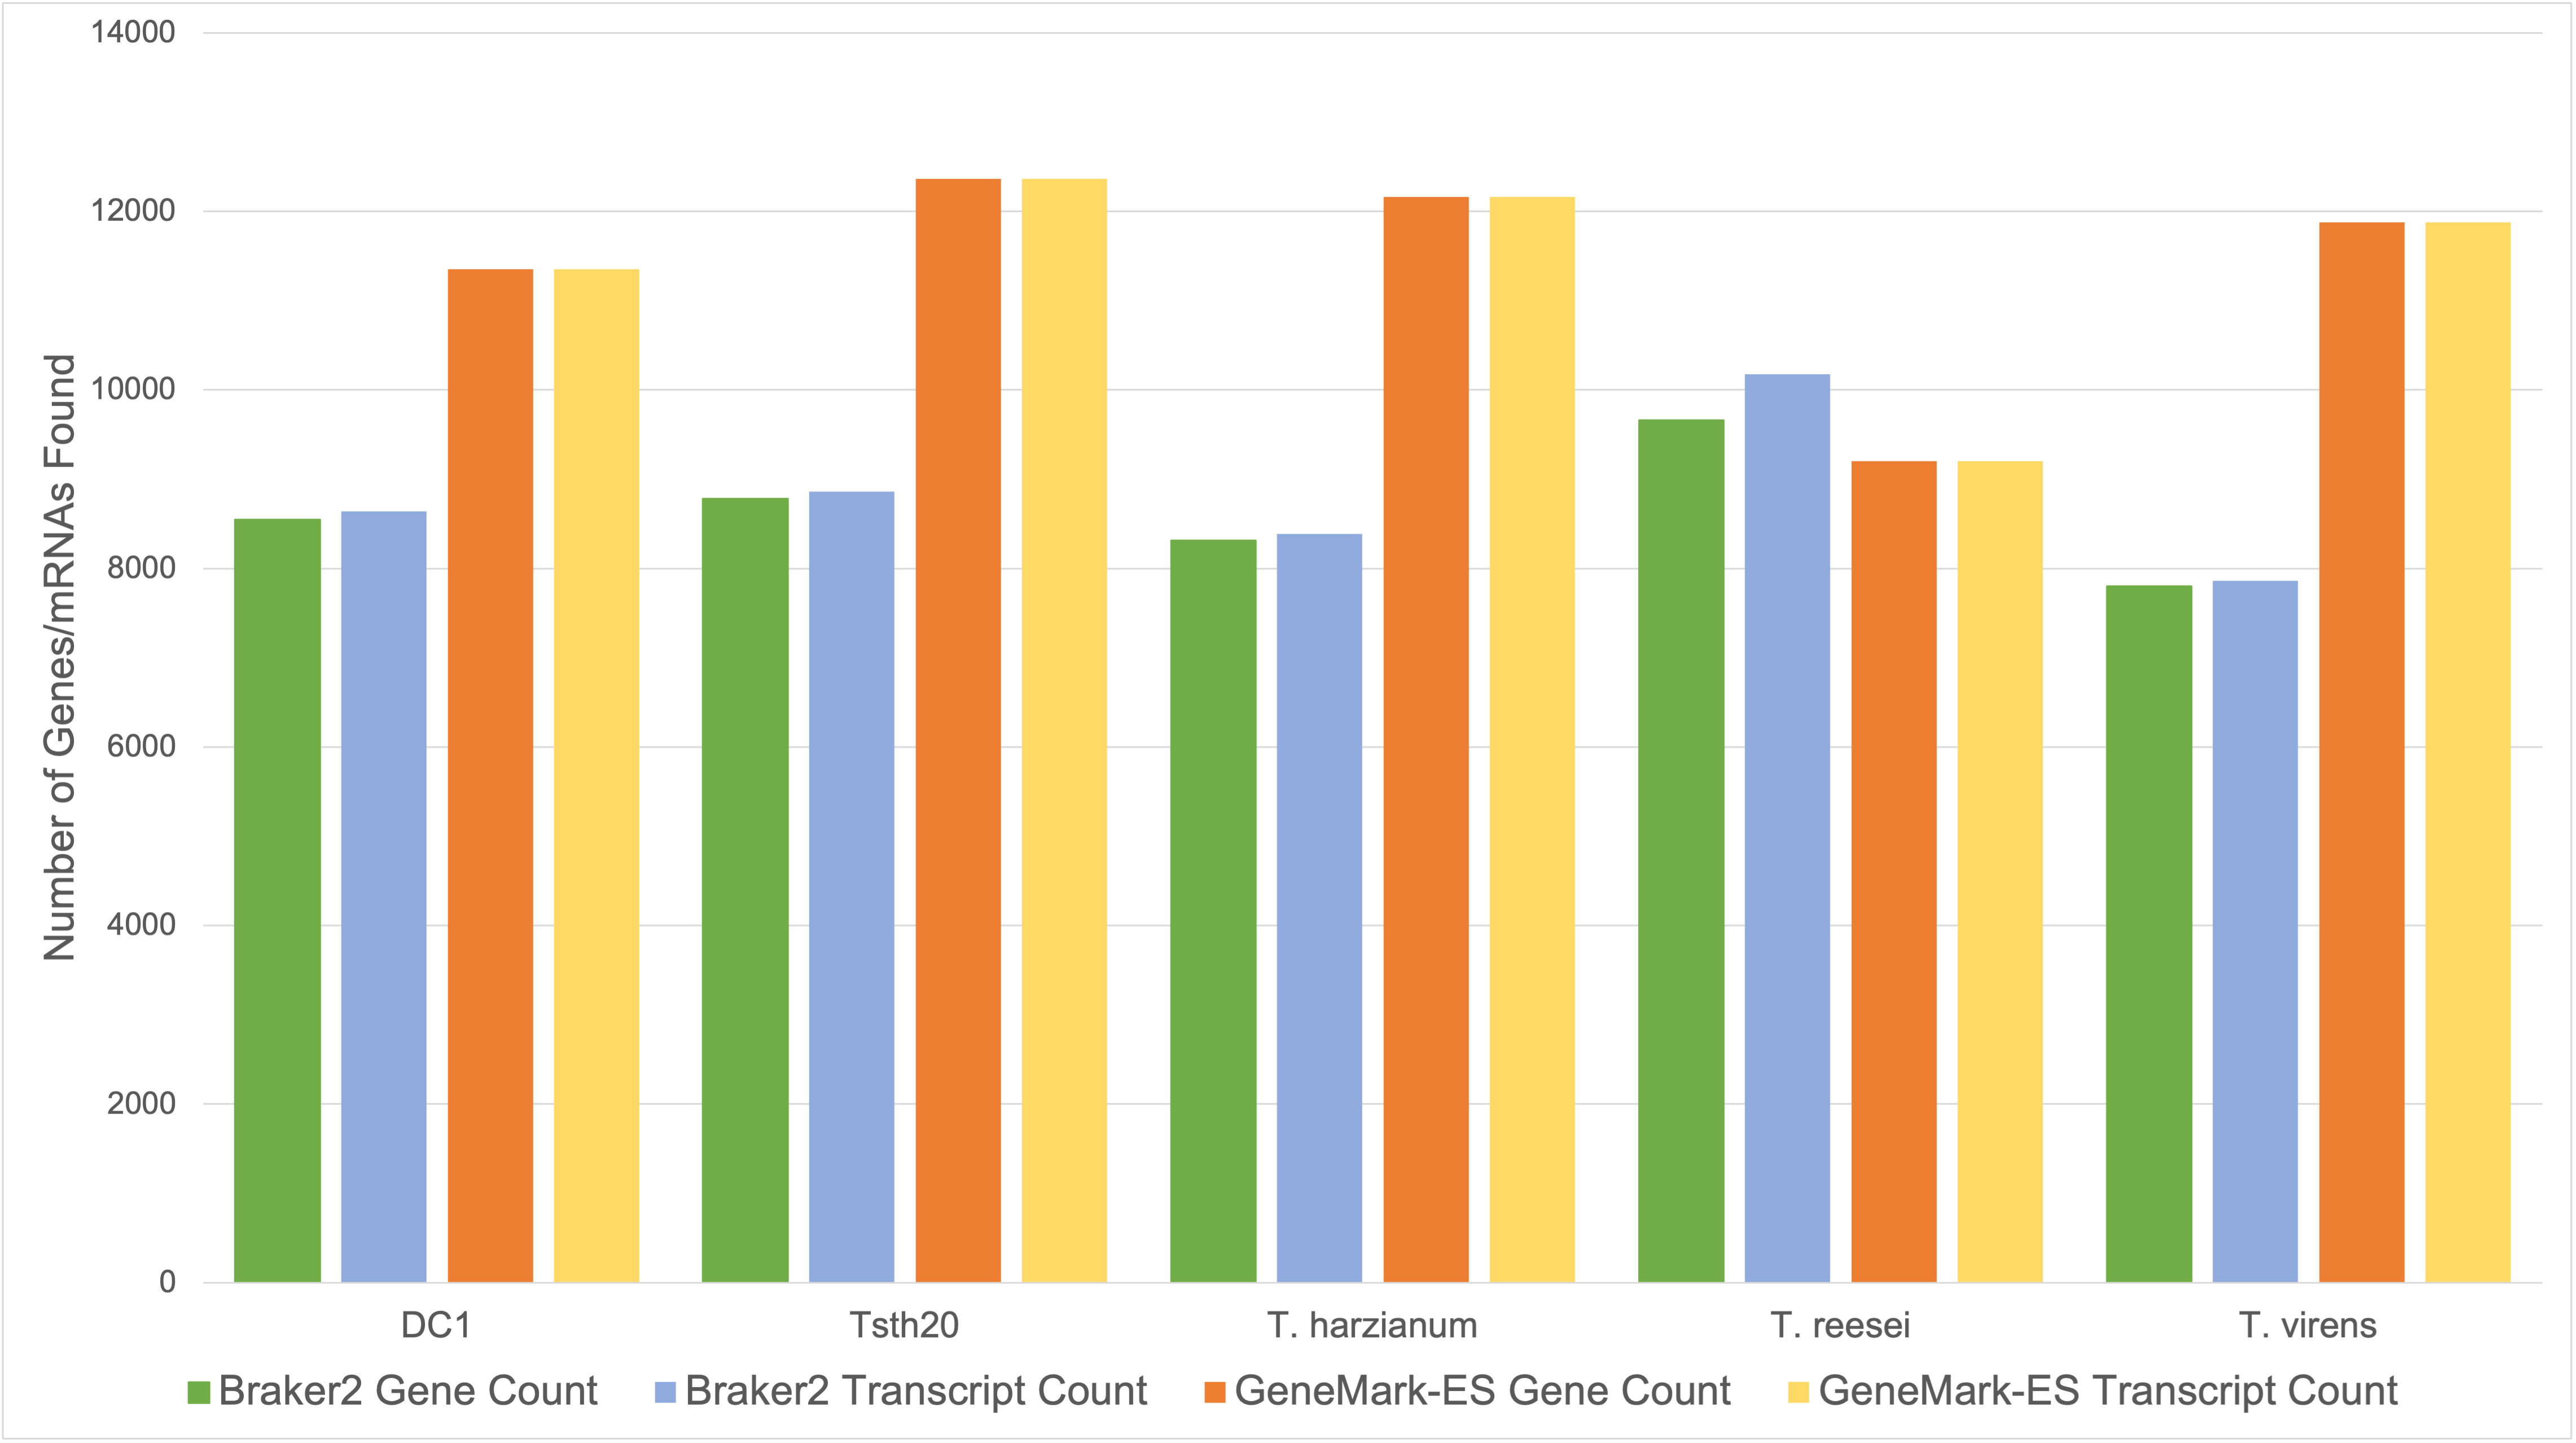
\includegraphics[width=\textwidth]{./figures/nextpolish-gene-finding.png}
  \caption{Shows the counts of genes and mRNAs found by each gene
    finding tool for each genome assembly considered.}
  \label{genecounts}
\end{figure}

One important ascpect to consider when looking at the output of
different gene prediction tools is the distribution of sequence
lengths predicted by any given tool. Lengths of possible sequences can
vary widely, ranging from small non-coding RNAs, which can be less
than 200 nucleotides in length, up to the largest genes which cover
more than two kilobases. Due to this wide variation in possible
sequence lengths, it is possible that different prediction tools could
produce different distributions of predicted sequence lengths. This is
important if researchers are interested in small non-coding RNAs or
atypically large genes. This section will investigate the coding
sequence lengths predicted by Braker and GeneMark for DC1 and Tsth20
while the RefSeq assemblies will also include the RefSeq annotation.

\section{Dsitribution of Predicted Gene Lengths}

In, gene finding tools will predict genes of different lengths within
a genome. To better understand the output produced by each gene
finder, we inspected the distributions of CDS lengths predicted by
each gene finding tool for each assembly. To better understand the
distribution of coding sequence (CDS) lengths produced by each gene
finding tool, running sums of CDS lengths proportional to the total
sum of CDS lengths were plotted and are visible in
figure~\ref{fig:cds-lengths}

\begin{figure}
  \centering
    \begin{subfigure}{0.8\textwidth}
      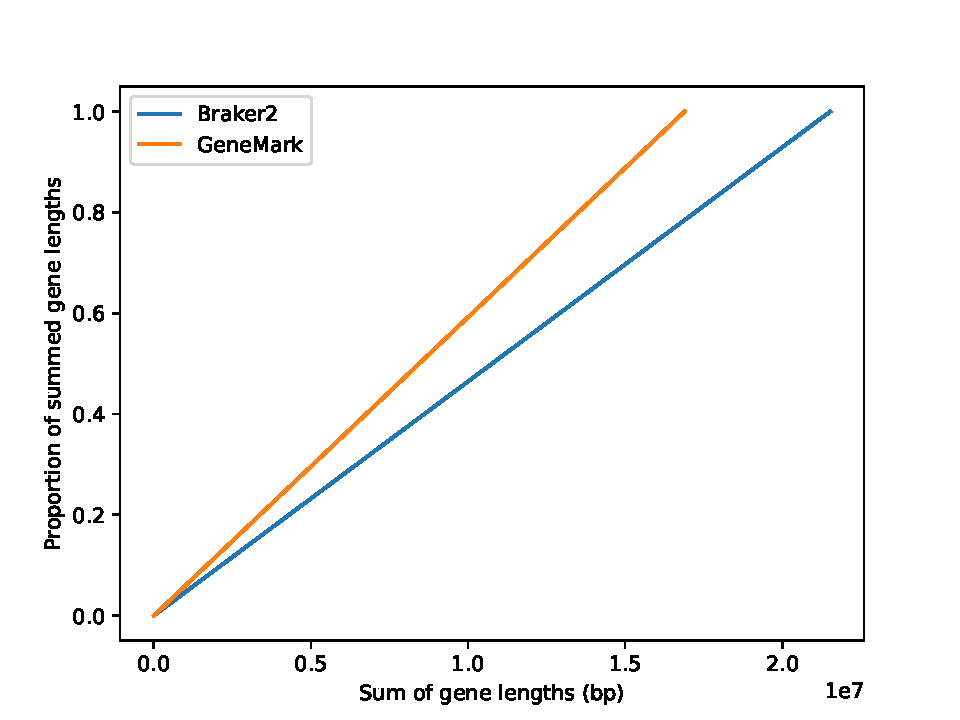
\includegraphics[width=\textwidth]{figures/dc1-cumulative-gene-lengths.pdf}
      \label{fig:dc1-lengths}
      \caption{DC1}
    \end{subfigure}
    \begin{subfigure}{0.8\textwidth}
      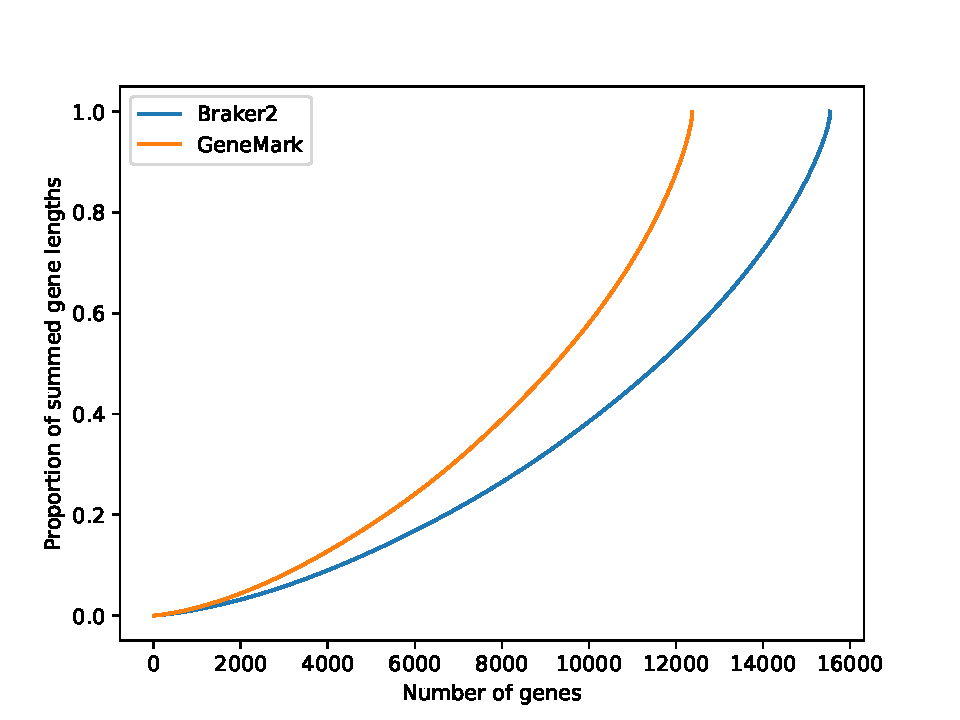
\includegraphics[width=\textwidth]{figures/tsth20-cumulative-gene-lengths.pdf}
      \label{fig:tsth20-lengths}
      \caption{Tsth20}
    \end{subfigure}
\end{figure}
\begin{figure}[ht]
  \ContinuedFloat
  \centering
    \begin{subfigure}{0.8\textwidth}
      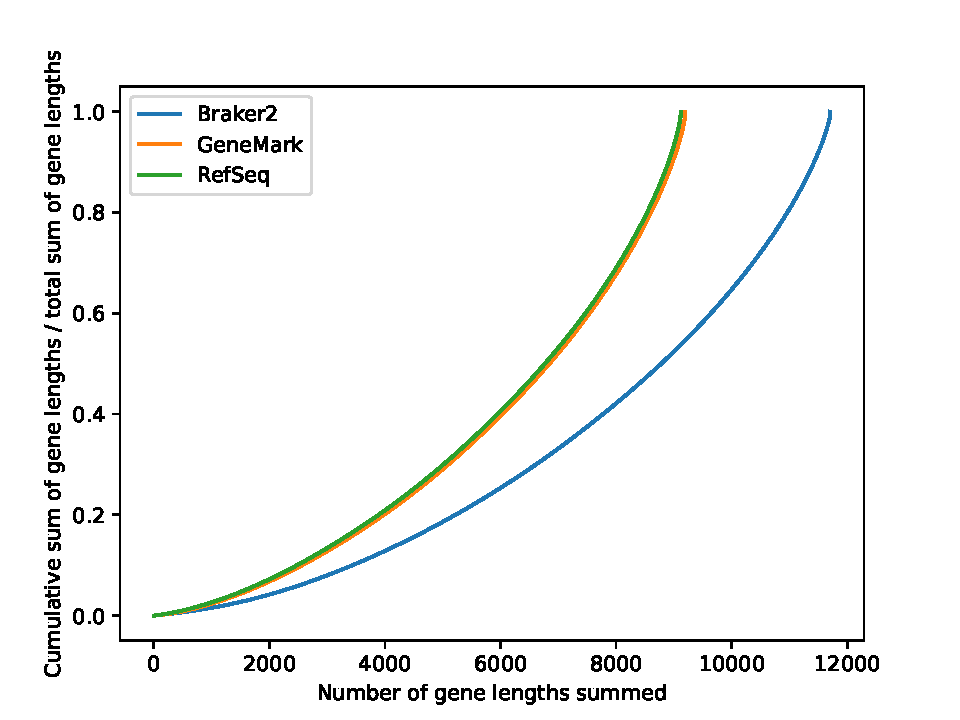
\includegraphics[width=\textwidth]{figures/t-reesei-cumulative-gene-lengths.pdf}
      \label{fig:treesei-lengths}
      \caption{\textit{T. reesei}}
    \end{subfigure}
    \begin{subfigure}{0.8\textwidth}
      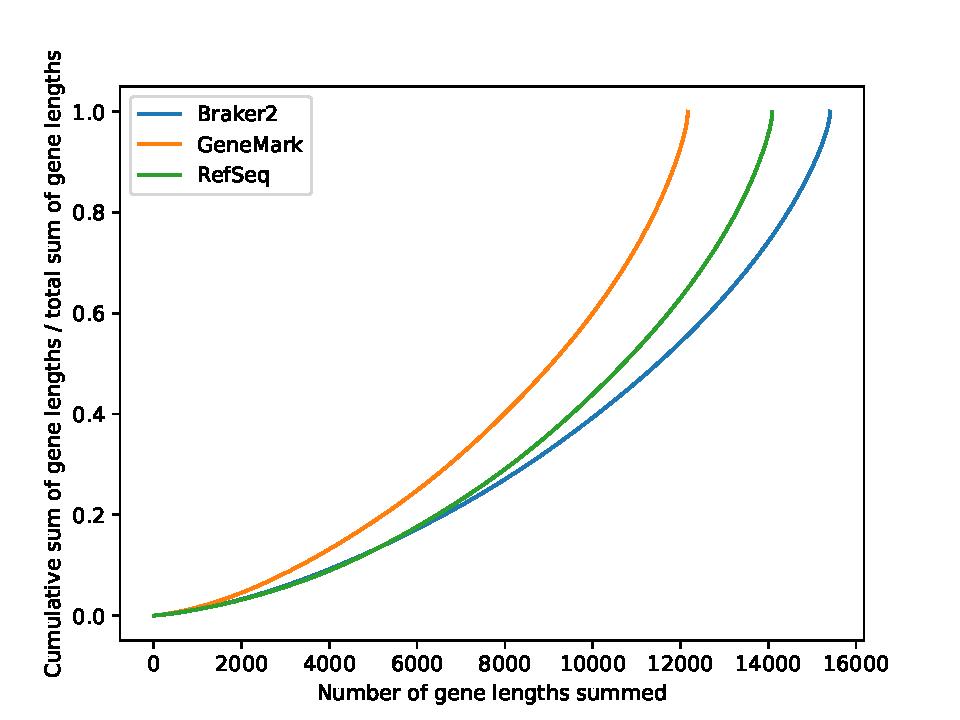
\includegraphics[width=\textwidth]{figures/t-harzianum-cumulative-gene-lengths.pdf}
      \label{fig:tharzianum-lengths}
      \caption{\textit{T. harzianum}}
    \end{subfigure}
\end{figure}
\begin{figure}[ht]
  \ContinuedFloat
  \centering
    \begin{subfigure}{0.8\textwidth}
      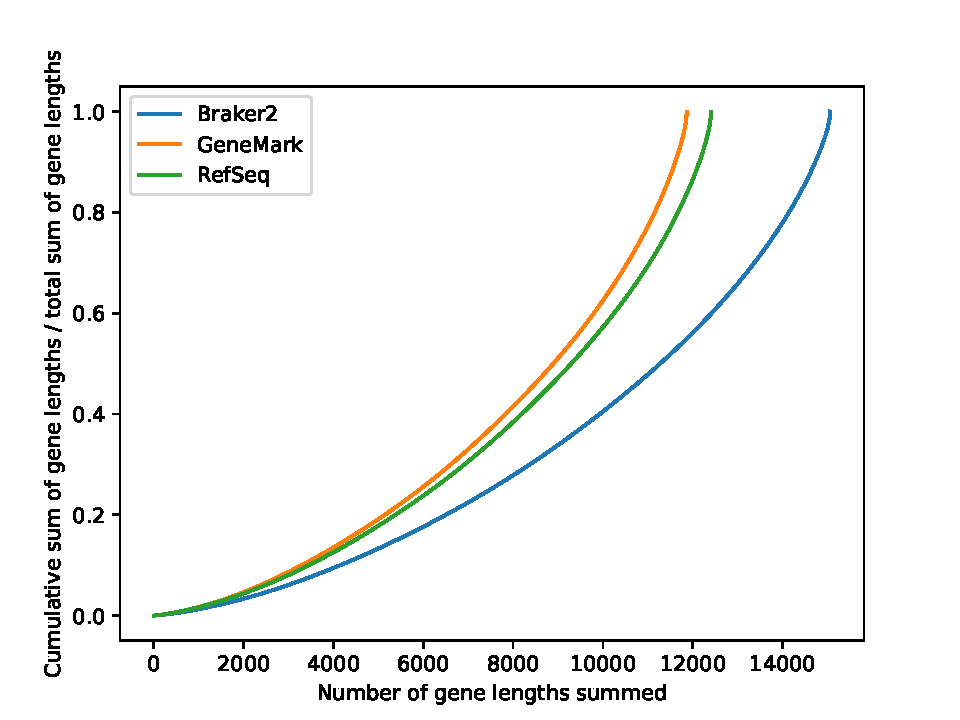
\includegraphics[width=\textwidth]{figures/t-virens-cumulative-gene-lengths.pdf}
      \label{fig:tvirens-lengths}
      \caption{\textit{T. virens}}
    \end{subfigure}
  \label{fig:cds-lengths}
  \caption{Running sums of CDS lengths proportional to total CDS
    length for each gene finding tool and assembly.}
\end{figure}
